
\begin{figure}[H]
    \centering
    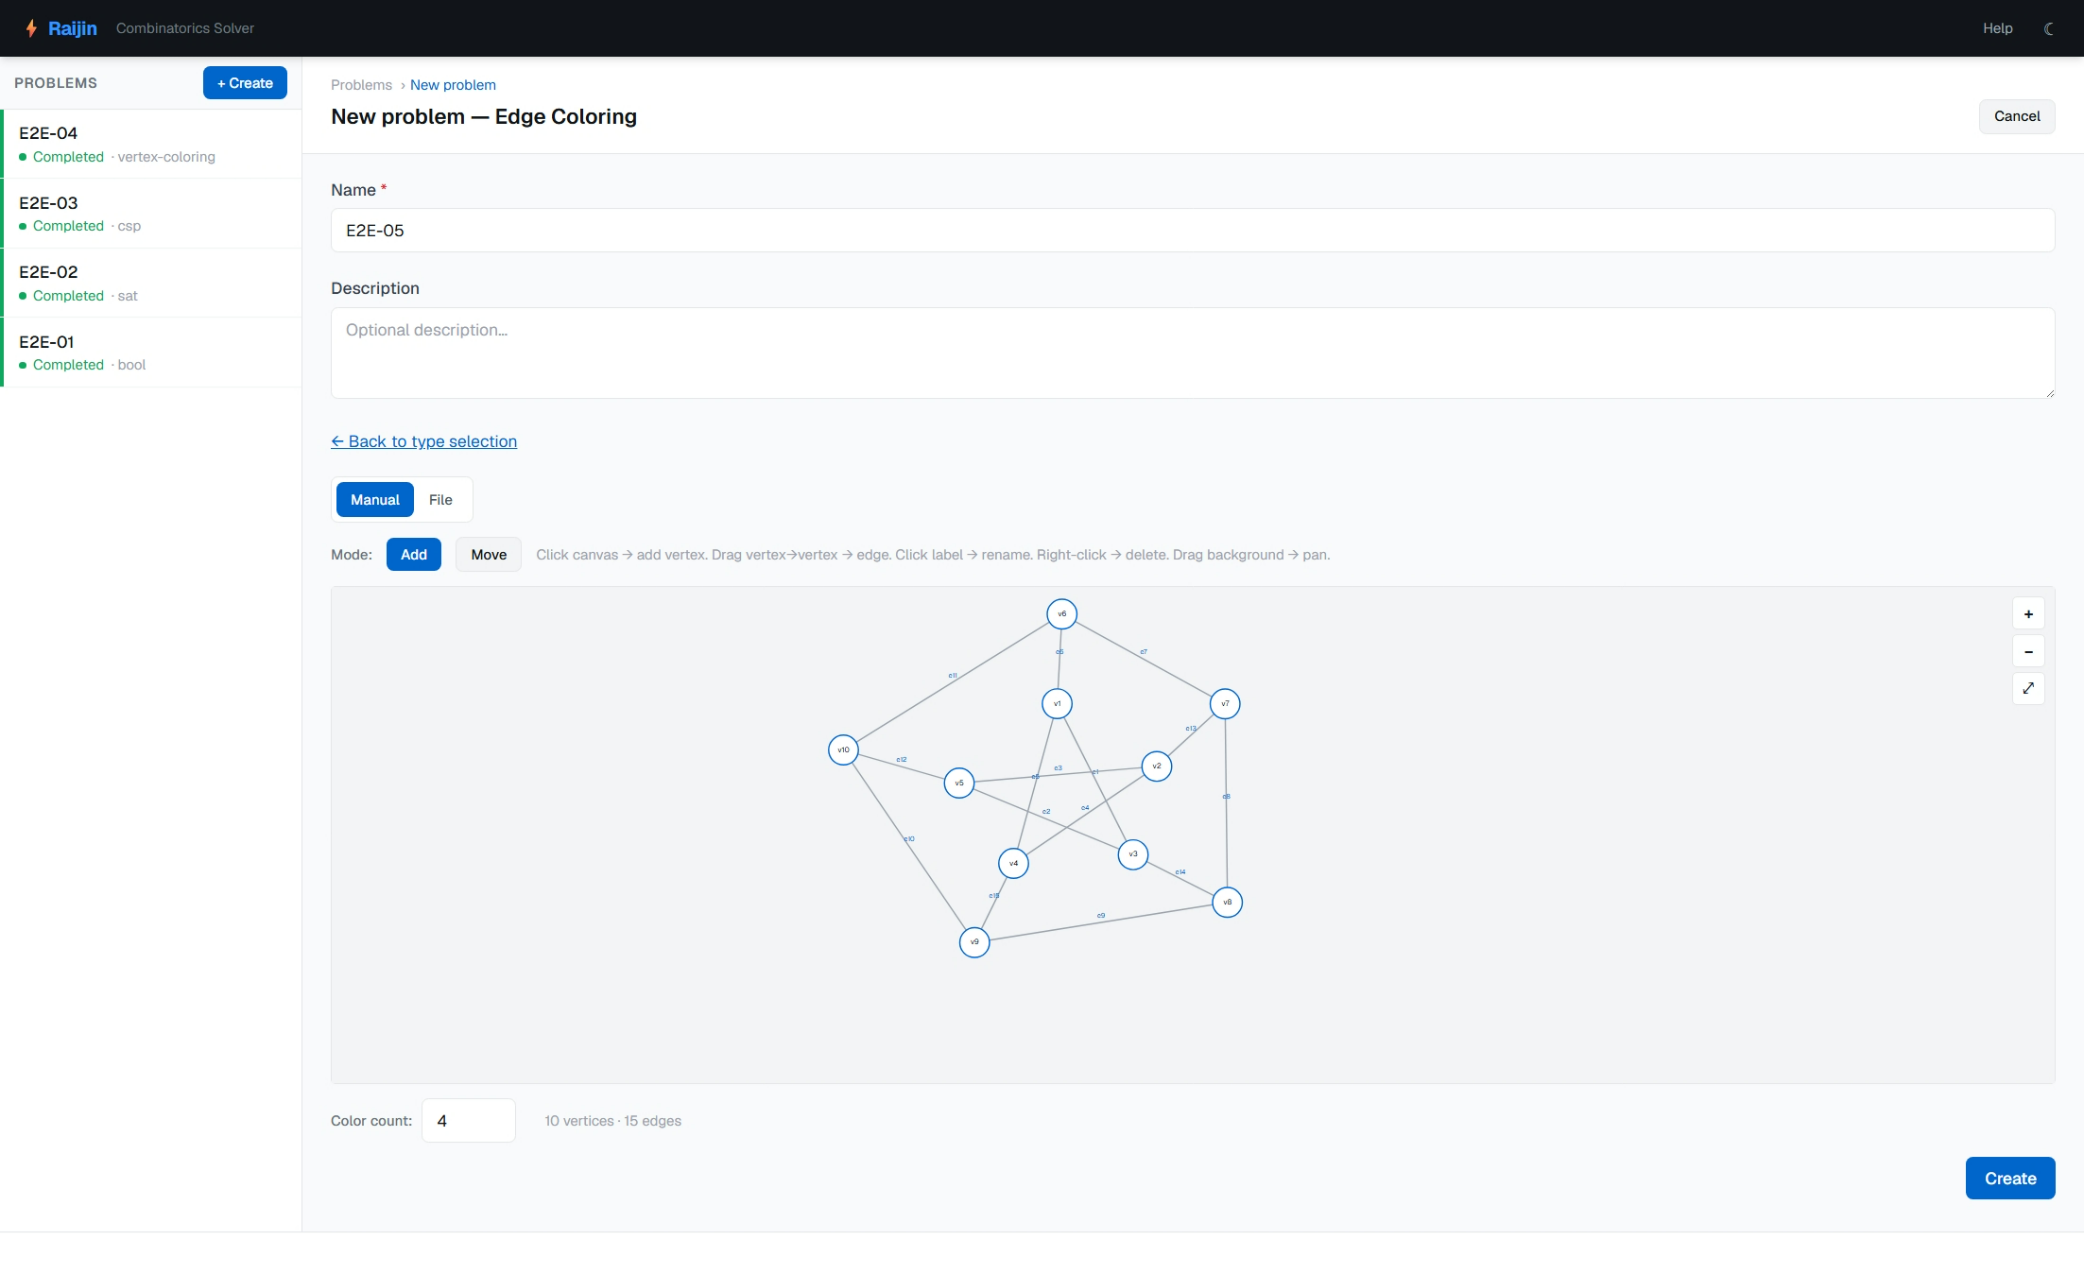
\includegraphics[width=\textwidth]{img/e2e-05-1.png}
    \caption{E2E-05 \ref{sec:testing:e2e-05}: Zadanie grafu na hranové farbenie (Petersenou graf; počet farieb je 4)}
    \label{fig:e2e-05-01}
\end{figure}

\begin{figure}[H]
    \centering
    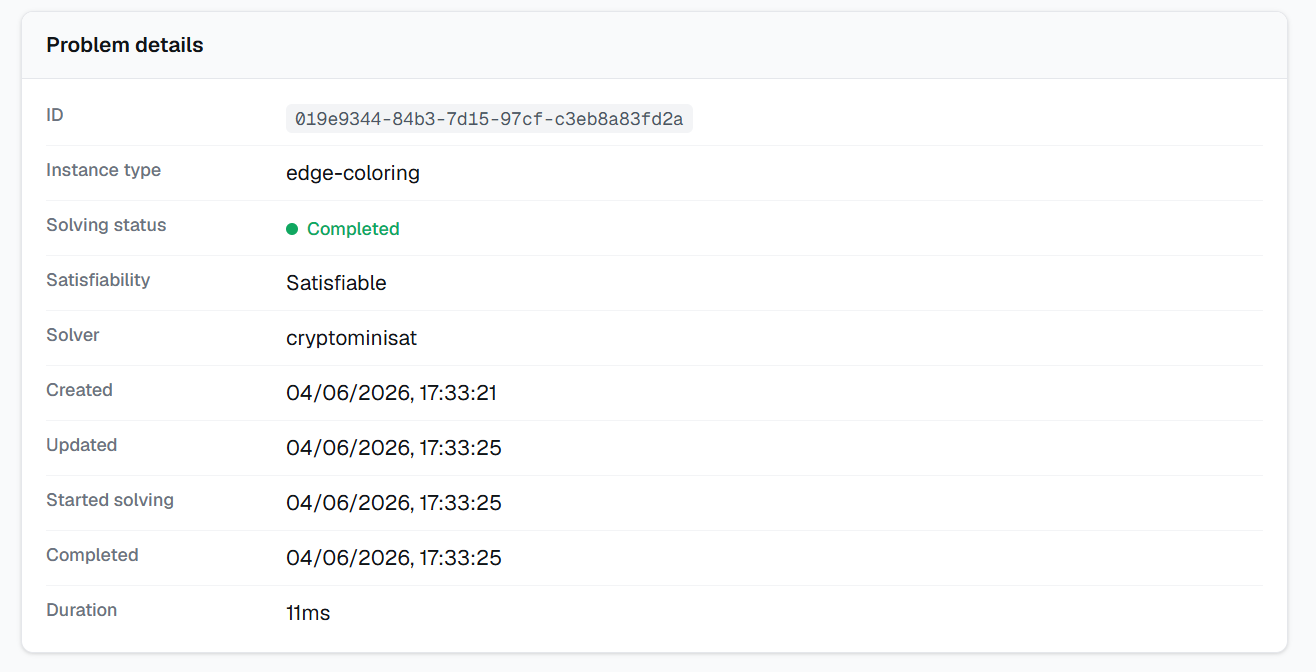
\includegraphics[width=\textwidth]{img/e2e-05-2.1.png}
    \caption{E2E-05 \ref{sec:testing:e2e-05}: Detail problému hranového farbenia grafu}
    \label{fig:e2e-05-02-01}
\end{figure}

\begin{figure}[H]
    \centering
    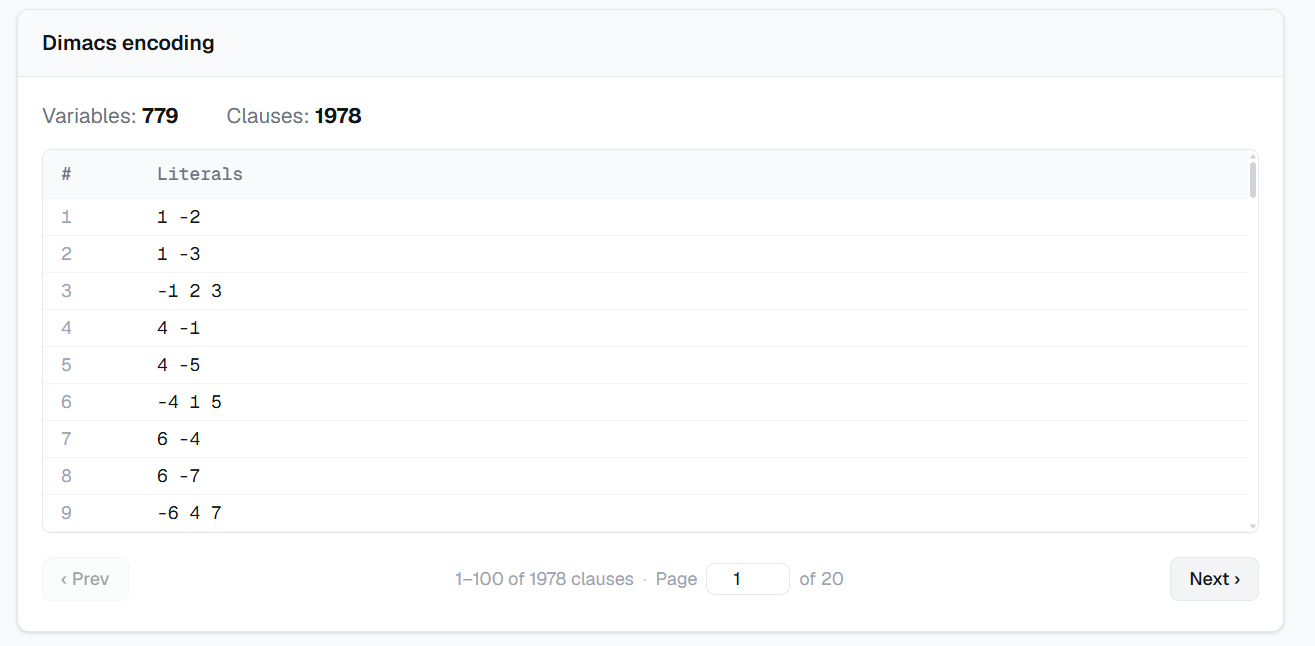
\includegraphics[width=\textwidth]{img/e2e-05-3.1.png}
    \caption{E2E-05 \ref{sec:testing:e2e-05}: Začiatok DIMACS kódovania problému hranového farbenia grafu}
    \label{fig:e2e-05-03-01}
\end{figure}

\begin{figure}[H]
    \centering
    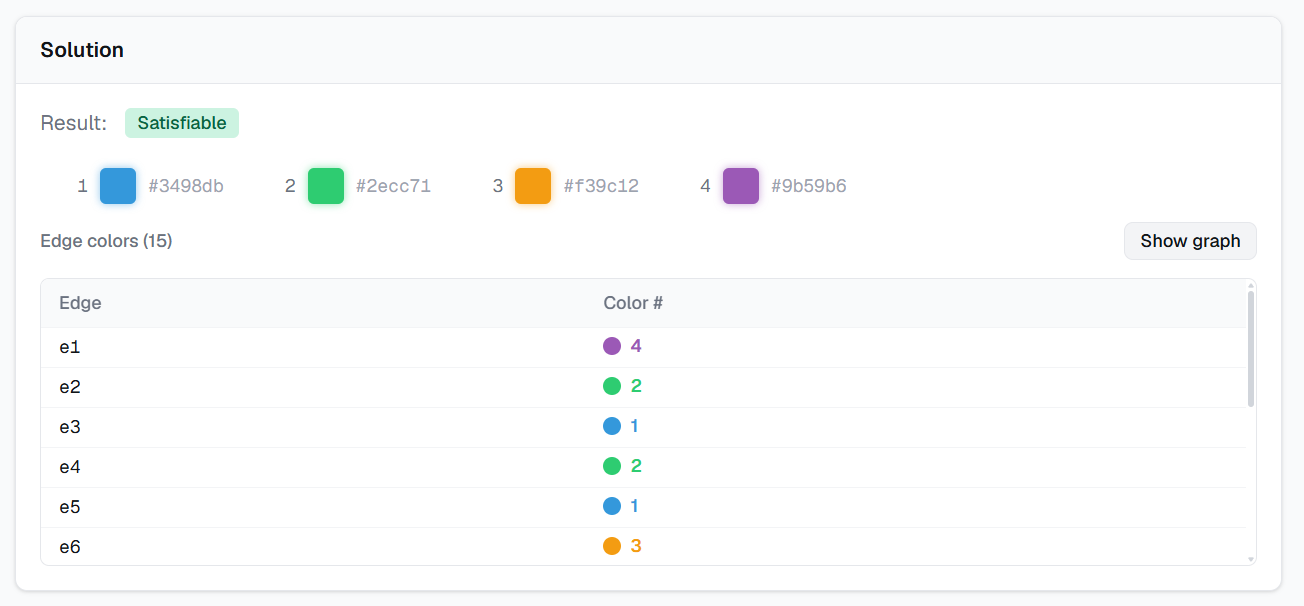
\includegraphics[width=\textwidth]{img/e2e-05-4.1.png}
    \caption{E2E-05 \ref{sec:testing:e2e-05}: Začiatok riešenia problému hranového farbenia grafu}
    \label{fig:e2e-05-04-01}
\end{figure}

\begin{figure}[H]
    \centering
    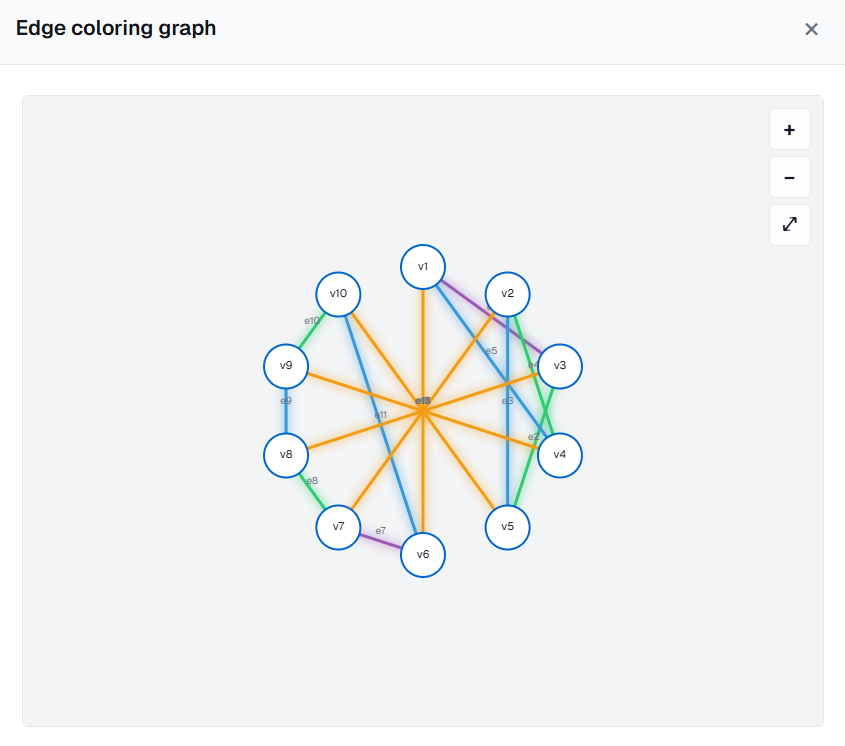
\includegraphics[width=\textwidth]{img/e2e-05-5.png}
    \caption{E2E-05 \ref{sec:testing:e2e-05}: Vizualizácia riešenia problému hranového farbenia grafu}
    \label{fig:e2e-05-05}
\end{figure}
